\onehalfspacing
\fancypagestyle{plain}{
\fancyhf{}
\rhead{\thepage}
\renewcommand{\headrulewidth}{0pt}
\renewcommand{\footrulewidth}{0pt}
}

\chapter{PLANTEAMIENTO}

\section{Antecedentes}

El panorama energético global atraviesa una fase crítica bajo el escenario de Ner Zero Emissions (NZE), impulsada por un cambio estructural donde la demanda total de energía disminuye un 7\,\% para 2030 respecto a los niveles de 2020 debido a mejoras drásticas en eficiencia, a pesar del crecimiento económico \citep{IEA_NZE_2021}. Sin embargo, la electrificación acelerada de sectores como el transporte y la industria redefine el consumo; se proyecta que la demanda eléctrica global crezca un 40\,\% para 2030, exigiendo que la intensidad energética de la economía mejore a una tasa anual del 4\,\% \citep{IEA_NZE_2021}.

De acuerdo con la hoja de ruta de la Agencia Internacional de Energía (IEA), este escenario marca el inicio de una era dominada por las energías limpias, donde el consumo eléctrico escala mientras que el suministro de energía primaria proveniente de combustibles fósiles cae del 80\,\% en 2020 a poco más del 20\,\% en 2050 (Véase Figura \ref{fig:TendenciasNZE2050}). Bajo el NZE, el despliegue de fuentes renovables debe ser masivo: para 2030, las adiciones anuales de energía solar fotovoltaica deben alcanzar los 630 GW y las de energía eólica los 390 GW, cuadriplicando el récord establecido en 2020. A pesar de que la energía solar y eólica se convierten en los pilares del sistema, la inversión anual en energía limpia debe aumentar desde los niveles actuales hasta alcanzar los 4 billones de dólares para 2030 \citep{IEA_NZE_2021}. Esta transición requiere superar cuellos de botella críticos, especialmente en la expansión y modernización de las redes eléctricas, cuya inversión anual debe duplicarse para evitar deficiencias en el balance energético y asegurar la integración de la generación variable, minimizando así el desperdicio forzado de energía limpia \citep{IEA_WEO_2025}.

\begin{figure}[H]
	% Fuerza la alineación izquierda y quita los ":" después del número
	\captionsetup{justification=raggedright, singlelinecheck=false, labelsep=none}
	
	\caption[Tendencias de la demanda energética proyectadas al 2050 bajo el escenario de Zero Net Emissions.]{} 
	
	% Vspace negativo opcional para acercar el texto cursivo al número de figura
	\textit{Tendencias de la demanda energética proyectadas al 2050 bajo el escenario de Zero Net Emissions.} \par\medskip
	
	\centering
	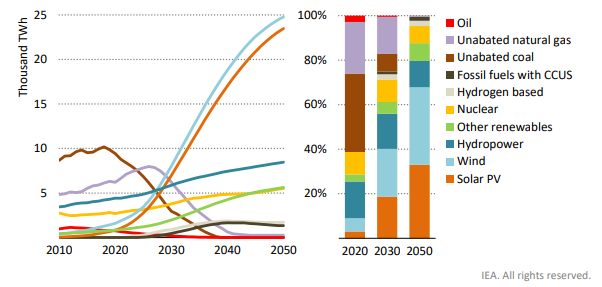
\includegraphics[width=0.8\textwidth]{Imagenes/NZE2050.png} \par\medskip
	
	\raggedright
	\footnotesize \textit{Nota.} Gráfico adaptado del reporte Net Zero Emissions by 2050 \citep{IEA_NZE_2021}.
	\label{fig:TendenciasNZE2050}
\end{figure}



En el ámbito nacional, la demanda energética peruana crece a un ritmo promedio del 3,5\,\% anual, con proyecciones sostenidas del 3\,\%, aunque evidencia una marcada disparidad regional \citep{ICEX2025}. Mientras que la zona centro reportó un incremento del 26\,\% en su demanda, las zonas norte y sur sufrieron contracciones del 36\,\% y 18\,\%, respectivamente.

En 2024, la producción eléctrica en el Perú alcanzó los 60.029 GWh, lo que supone un crecimiento del 3\,\%. Si bien la matriz nacional mantiene un sólido respaldo en fuentes hidráulicas y térmicas, las energías renovables no convencionales ganan terreno progresivamente \citep{ProActivo2025}. Para octubre de 2025, la generación mediante recursos renovables (solar, eólica, bagazo y biogás) creció un 27\,\% interanual, alcanzando el 13\,\% de la producción total. El objetivo estratégico del Estado es profundizar esta transición hasta que las energías limpias constituyan el 20\,\% de la matriz para el año 2030.

Las nuevas tendencias energéticas, lideradas por la tecnología solar fotovoltaica, plantean retos técnicos complejos para garantizar la eficiencia operativa \citep{XPower2024}. A medida que los proyectos fotovoltaicos escalan y se sitúan en terrenos topográficamente irregulares, factores como la variabilidad espacial de la irradiancia, las fluctuaciones térmicas, la suciedad y el ensombrecimiento afectan directamente la producción \citep{Salinas2025}. Bajo este escenario, la instrumentación rigurosa se convierte en un componente crítico \citep{SevenSensor}. El despliegue estratégico de redes de sensores, equipos de diagnóstico y plataformas de monitoreo continuo es indispensable para determinar el índice de rendimiento (\textit{Performance Ratio}) bajo normativas como la IEC 61724 \citep{IEC61724-1_2021}. Esta precisión no solo valida el diseño de la planta frente a la variabilidad climática, sino que habilita estrategias de mantenimiento predictivo capaces de anticipar anomalías, minimizar tiempos de inactividad y asegurar el retorno de inversión, consolidando a la energía solar como una infraestructura económica y resiliente \citep{Anatrac}.

\section{Definición de la problemática}

La implementación de instrumentación en plantas fotovoltaicas se enfrenta a un desafío logístico y técnico considerable: la heterogeneidad de las condiciones climáticas dentro de una misma instalación \citep{Salinas2025}. A medida que los proyectos a gran escala se asientan sobre terrenos con topografías complejas, como las vistas en la Figura \ref{fig:PlantaPeru}, se generan microclimas que provocan variaciones espaciales significativas. Por ejemplo, las diferencias de elevación alteran localmente los perfiles aerodinámicos del viento, mientras que las variaciones del albedo y el sombreado dinámico causan una distribución desigual de la radiación solar. Estudios en plantas de gran tamaño demuestran que esta dispersión geográfica puede generar diferencias de hasta un 20\,\% en la irradiación diaria y más del 40\,\% a nivel horario, así como variaciones térmicas de 6 a 7 °C entre paneles separados por unos pocos cientos de metros \citep{Garcia2014}.


\begin{figure}[H]
	% Fuerza la alineación izquierda y quita los ":" después del número
	\captionsetup{justification=raggedright, singlelinecheck=false, labelsep=none}
	
	\caption[Imagen aérea de planta de energía solar en inmediaciones de la fábrica de cemento Yura, Arequipa.]{} 
	
	\textit{Imagen aérea de planta de energía solar en inmediaciones de la fábrica de cemento Yura, Arequipa.} \par\medskip
	
	\centering
	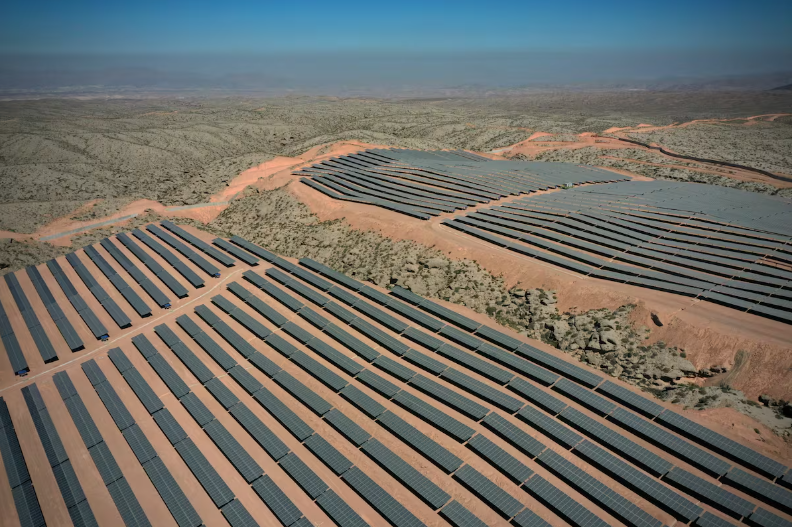
\includegraphics[width=0.6\textwidth]{Imagenes/PlantaPeru.png} \par\medskip
	
	\raggedright
	\footnotesize \textit{Nota.} Fotografía adaptada sobre la noticia ``Yura y el poder del sol'' \citep{YuraPeru}.
	\label{fig:PlantaPeru}
\end{figure}

Para hacer frente a esta variabilidad y cumplir con los requisitos de monitorización de normativas internacionales, como la IEC 61724-1 \citep{IEC61724-1_2021}, las plantas recurren actualmente a la instalación de estaciones  meteorológicas y redes de instrumentación fija. En el contexto de un parque fotovoltaico, una estación meteorológica se concibe como un núcleo de monitorización centralizado mediante un adquisidor de datos, el cual integra una serie de instrumentos de alta precisión para caracterizar el recurso solar y el entorno climático \citep{Anatrac}. Típicamente, esta estación está equipada con piranómetros, sensores de temperatura ambiente, anemómetros y medidores de humedad relativa y presión atmosférica.\citep{ProyectoEjecutivo2024}. Sin embargo, depender exclusivamente de puntos de medición estáticos presenta severas limitaciones. En la práctica, unos pocos sensores no logran capturar con precisión la variabilidad climática real a lo largo de terrenos extensos y con seguidores solares en dinámica constante \citep{Salinas2025}.

En consecuencia, el problema central se define como la ineficiencia de los métodos de instrumentación estáticos para caracterizar adecuadamente la variabilidad climática a lo largo de una planta fotovoltaica. Dado que resulta logísticamente inviable instalar estos instrumentos fijos en cada fila de paneles, los operadores se enfrentan a una alta incertidumbre en la evaluación de los índices de rendimiento energético y a deficiencias importantes para la detección y localización oportuna de fallas. 

A esta falta de representatividad espacial se suma el desafío financiero de intentar escalar o densificar la red de monitoreo, lo que representa gastos que llegan a constituir hasta el 1,6\,\% del presupuesto total de inversión de una planta fotovoltaica \citep{Burriana5MW}. Este conjunto de barreras evidencia la necesidad urgente de transitar hacia métodos de inspección dinámicos y verdaderamente representativos de todo el entorno solar.

%NOTA: AGREGAR MÁS CONSECUENCIAS, APARTE DE COSTOS, QUÉ MÁS?

\section{Propuesta de solución}
Para superar las limitaciones del monitoreo convencional, esta propuesta plantea el diseño y desarrollo de un robot autónomo especializado en la medición dinámica de variables climáticas dentro de sistemas fotovoltaicos. A diferencia de la infraestructura fija, este sistema funciona como una plataforma móvil adaptada para transportar instrumentos meteorológicos, lo que le permite realizar un barrido continuo en diversas secciones de la planta. Al desplazarse estratégicamente por el terreno, el robot recolecta datos que reflejan con mayor exactitud la dispersión geográfica de la irradiancia, los microclimas y las condiciones ambientales locales, con el fin de reducir el error en el cálculo y la estimación de la generación de energía, en cumplimiento con los métodos y exigencias de las normativas internacionales. Para complementar su funcionalidad, el sistema está diseñado para almacenar y transmitir toda la información capturada de forma inalámbrica, facilitando una plataforma de monitoreo remoto donde los operadores pueden visualizar el estado ambiental de la planta en tiempo real.


\subsection{Objetivos generales}

\subsubsection{Objetivo correspondiente a Trabajo de Fin de Carrera 1 (1MTR01)}
Elaborar el diseño conceptual y el anteproyecto de un robot autónomo para la medición de variables climáticas en sistemas fotovoltaicos.

\subsubsection{Objetivo para el proyecto general}
Desarrollar y elaborar el proyecto definitivo e implementar un prototipo del robot autónomo para la medición de variables climáticas en sistemas fotovoltaicos.

\subsection{Objetivos específicos}

\subsubsection{Objetivos correspondientes a Trabajo de Fin de Carrera 1 (1MTR01)}
\begin{itemize}
    \item Determinar los requerimientos funcionales, cinemáticos y de diseño del sistema mecatrónico a partir del análisis de las condiciones topográficas y climáticas en los parques solares.
    \item Desarrollar el diseño conceptual del sistema de locomoción, identificando sus funciones mecánicas y seleccionando los principios de tracción óptimos para garantizar un desplazamiento estable sobre terrenos irregulares.
    \item Desarrollar el diseño conceptual del mecanismo articulado, abstrayendo sus requerimientos cinemáticos y de actuación para asegurar la orientación independiente y precisa de los sensores climáticos.
    \item Estructurar la lógica del sistema de control autónomo, definiendo las funciones de procesamiento de señales, navegación y actuación requeridas para el seguimiento de rutas y la evasión de obstáculos.
    \item Plantear la arquitectura para el subsistema de telemetría y comunicaciones para garantizar la transmisión confiable de datos entre el robot y la central de control.
    \item Seleccionar el concepto de solución óptimo del sistema mediante una evaluación técnico-económica de las diferentes alternativas planteadas.
\end{itemize}

\subsubsection{Objetivos para el proyecto general}
\begin{itemize}
    \item Diseñar a detalle una base de transporte con alta capacidad de tracción, a partir del concepto mecánico seleccionado, para operar de manera estable sobre los terrenos irregulares que caracterizan a los parques solares.
    \item Diseñar una base móvil articulada e integrada al vehículo, basándose en la arquitectura óptima definida previamente, capaz de moverse y orientarse de forma independiente para adaptarse a la posición óptima requerida por los diversos sensores ambientales.
    \item Desarrollar un algoritmo de control autónomo, implementando la lógica estructurada en el diseño conceptual, que proporcione al vehículo la inteligencia necesaria para seguir rutas de inspección predefinidas y reaccionar ante imprevistos mediante la evasión de obstáculos.
    \item Implementar una infraestructura de comunicación inalámbrica, materializando el esquema tecnológico propuesto, utilizando paneles solares para energizar de forma autónoma los puntos independientes de comunicación, garantizando que los datos recolectados lleguen al centro de control sin interrupciones y permitiendo la intervención manual remota.
    \item Elaborar el proyecto definitivo del sistema incluyendo la elaboración de la lista de materiales, la estimación total de costos de implementación y la planificación de los protocolos de mantenimiento.
\end{itemize}

\section{Alcance y limitaciones}
El alcance de este proyecto y sus delimitaciones operativas se definen en conjunto a través de las siguientes características:

\begin{itemize}
    \item Abarca el diseño de detalle y la implementación de un prototipo físico o virtual de una base móvil robusta apta para desplazarse sobre los terrenos irregulares que caracterizan a las plantas fotovoltaicas.
    
    \item Incluye el desarrollo de la lógica y el algoritmo de control que permitirá al vehículo seguir rutas de inspección predefinidas y evadir obstáculos. No obstante, el desplazamiento se encuentra restringido por la morfología del suelo, limitando su operación a zonas con pendiente máxima del terreno de $14^\circ$.
    
    \item Comprende la incorporación de los instrumentos meteorológicos requeridos para monitorear las variables ambientales de forma dinámica. La precisión de esta instrumentación estará sujeta a factores ambientales, pudiendo verse mermada por el fenómeno del \textit{soiling} o presentar lecturas atípicas debido a sombras proyectadas y reflejos solares accidentales.
    
    \item La integridad mecánica, electrónica y de los sensores del sistema estará diseñada para soportar las altas exigencias climáticas de los parques solares, restringiendo su funcionamiento seguro a una temperatura ambiente máxima operativa de 45\,$^\circ$C.
    
    \item Contempla la implementación de un sistema de telemetría para almacenar y transmitir los datos medidos, habilitando la supervisión y el control remoto. Su desempeño dependerá estrictamente de la cobertura y estabilidad de la red inalámbrica existente en la instalación.
    
    \item La autonomía del robot estará directamente condicionada por la capacidad de su batería y su perfil de consumo energético, proyectándose una autonomía de operación continua de alrededor de 4 horas, lo que impone la necesidad de establecer ciclos de carga periódicos para mantener la continuidad del servicio en plantas que requieran un recorrido mayor al tiempo establecido..
\end{itemize}

\section{Metodología del diseño} 

El desarrollo del sistema mecatrónico se guiará por la directriz VDI 2221. Aunque la Ingeniería de Sistemas Basada en Modelos (MBSE) es una alternativa moderna que emplea modelos digitales formales para simular y analizar todo el ciclo de vida \citep{Isdefe2023}, su implementación requiere un ecosistema de software complejo orientado principalmente a sistemas de sistemas de alta criticidad. Por ello, se ha seleccionado la VDI 2221 para esta etapa del proyecto. En contraste con la MBSE, la norma VDI ofrece un enfoque pragmático y secuencial, perfectamente alineado con los objetivos del curso. De acuerdo con el cronograma del proyecto, el proceso se ha dividido en las siguientes fases:

\subsection{Definición de la tarea} 
Abarcada en los primeros avances del cronograma, esta fase involucra la recolección y el análisis exhaustivo de las condiciones operativas, topográficas y climáticas reales de los parques fotovoltaicos. Durante esta etapa se elabora el estado del arte, analizando las limitaciones de la instrumentación fija actual y los vehículos de inspección existentes. La fase culmina con la redacción de la lista de requerimientos, donde se determinan y cuantifican los requerimientos funcionales, cinemáticos y de diseño obligatorios para el sistema mecatrónico.

\subsection{Diseño conceptual} 
Desarrollada a través de entregas progresivas, esta fase materializa el enfoque modular establecido en los objetivos del proyecto. Inicia con la abstracción de la problemática mediante una caja negra y la definición de la estructura de funciones general. A partir de ello, el diseño se divide en los cuatro subsistemas clave: el sistema de locomoción, el mecanismo articulado, el sistema de control autónomo y el subsistema de telemetría y comunicaciones. Las funciones de estos subsistemas, a su vez, se clasifican en dominios. Para cada dominio se elaboran matrices morfológicas independientes. Finalmente, al integrar estos portadores de funciones, se proponen distintas alternativas conceptuales del robot, las cuales se someten a una evaluación técnico-económica para seleccionar el concepto de solución óptimo, presentando el anteproyecto a través de un modelo 3D.

\subsection{Diseño de detalle} 
Ubicada en la etapa de proyecto definitivo del cronograma, constituye la última etapa del desarrollo constructivo, en la cual se fijan con precisión las dimensiones, geometrías, presupuesto y la Lista de Materiales del sistema. Aquí se genera toda la documentación técnica requerida para la manufactura y puesta en marcha del robot autónomo, abarcando tres áreas clave: 

\begin{itemize} 
    \item \textbf{Dominio mecánico:} Elaboración de planos de fabricación, selección de materiales y dimensionamiento estructural definitivo tanto de la base móvil de tracción como de la base articulada de soporte para los sensores. 
    \item \textbf{Dominio electrónico y de energía:} Diseño de esquemáticos, enrutamiento de placas de circuito impreso, integración de la instrumentación de variables climáticas y dimensionamiento del sistema de alimentación independiente. 
    \item \textbf{Dominio de control y comunicaciones:} Desarrollo de la arquitectura de algoritmos para el seguimiento de rutas y evasión de obstáculos y diseño del enlace inalámbrico que garantizará la transmisión de datos al centro de monitoreo. 
\end{itemize}

\subsection{Implementación digital y validación}
Correspondiente a la etapa final de implementación del cronograma, esta fase se define de manera estrictamente digital, descartando la construcción física y enfocándose en el desarrollo de un prototipo virtual del diseño propuesto. Bajo este entorno digital, el proceso de validación se centrará única y exclusivamente en comprobar el sistema de comunicación inalámbrica. A través de herramientas de integración de red y simulación, se evaluará que el enlace de telemetría y la transmisión de los datos climáticos hacia la estación de monitoreo sean estables, asegurando que la arquitectura de red no sufra interrupciones y satisfaga todos los parámetros de conectividad estipulados en la lista de requerimientos.